\chapter{Deep Fractal based Hashing - DAsH}
 
 

\section{Consideraciones Iniciales}

La creciente disponibilidad de datos en diversos dominios ha creado la necesidad de desarrollar técnicas y métodos para descubrir el conocimiento a partir de volúmenes masivos de datos complejos, motivando a muchos investigadores a trabajar en \textit{databases, machine learning}, y comunidades de recuperación de información. Esto ha impulsado el desarrollo de técnicas escalables y eficientes para organizar y recuperar este tipo de datos. Las búsquedas por similitud han sido el enfoque tradicional para la recuperación de la información. Considerando que la similitud es el criterio instintivo por el cual las personas hacen comparaciones, las comunidades de recuperación de información usan similitud para organizar y buscar datos.    Sin embargo, la similitud es una medida intuitiva para la comparación, causa algunas dificultades en representar datos complejos y con la estabilidad de los algoritmos cuando la dimensionalidad de los datos es muy alta (la ``maldición de la dimensionalidad''). Aunque muchos trabajos de investigación se han llevado a cabo en el desarrollo de estructuras eficientes de índices y algoritmos de búsqueda por similitud, sólo unos pocos presentan una garantía teórica de estabilidad asintótica para datos de alta dimensión.

Uno de los pocos enfoques que aseguran una solución aproximada con el coste de búsqueda sublineal para datos de alta dimensión es \textit{Locality Sensitive Hashing} (LSH) \cite{lsh}.LSH se basa en la idea de que la cercanía entre dos objetos suele ser preservada por una operación de proyección aleatoria. En otras palabras, si dos objetos están cerca juntos en su espacio original, entonces estos dos objetos permanecerán cerca después de una operación de proyección escalar. Sin embargo, presenta algunas dificultades para consultas kNN aproximadas, en particular, relacionadas con la dependencia de los parámetros del dominio de los datos y resultados de calidad. Por lo tanto, en dominios complejos, en particular, en problemas con datos con gran dimensión, una solución aproximada con un sólido análisis teórico puede ser la mejor opción en muchas áreas de aplicación debido a su eficiencia en tiempo y espacio.

Por otra parte, en \textit{Machine Learning} las imágenes se describen a menudo mediante las características visuales manuales.  Sin embargo, estas características manuales no pueden revelar el significado semántico de alto nivel (etiquetas o tags) de las imágenes, y a menudo limitan el rendimiento de la recuperación de imágenes \cite{Li:2015:RSS:2881665.2882186}. Así, para obtener esta información semántica tenemos que trabajar con la información de la etiqueta y procesar los datos en un modo supervisado. Inspirado por recientes avances en \acf{CNN} para problemas de clasificación de imágenes, detección de objetos, y muchas otras tareas de visión \cite{ImageNet,NIPS2013_5207,LiuWJJC12}, muchos métodos resolvieron el problema de la precisión de la recuperación de similitud utilizando CNN como extractor de características y luego construir un código hash compacto de preservación de similitud para la recuperación rápida de imágenes.   De nuevo, \textit{hashing} es ampliamente usado para recuperar imágenes a gran escala así como las búsquedas de video y documentos porque la representación compacta del código hash es esencial para el almacenamiento de datos y es razonable para las búsquedas de consultas \cite{conf/cvpr/ShenSLS15}.  Sin embargo, algunos inconvenientes basados en estos métodos de \textit{hashing} supervisados no se han resuelto completamente, como sigue:


\begin{itemize}

\item[-]  Existe una compensación entre error de clasificación y error de cuantificación: activaciones de capas inferiores son más generales \cite{DBLP:journals/corr/YosinskiCBL14}, así que el entrenamiento es más eficaz. Sin embargo, las capas inferiores tienen mapas de activaciones más grandes (muchos nodos), las cuales son más difíciles de codificar, lo que conduce a un compromiso. 
	
 
\item[-] Existe una dependencia de los valores de los parámetros para esquemas aproximados de búsqueda de similitud basados en LSH, que determinan el número de funciones hash y el número de tablas hash.  
 
\end{itemize}

En este tesis  se propone una nueva técnica de \textit{hashing} supervisada,  llamada  \textit{Deep frActal based  Hashing} (DAsH),  diseñado para realizar una búsqueda de similitud aproximada escalable. Las contribuciones de nuestro trabajo son las siguientes. Primero,  introducimos y definimos un esquema jerárquico basado en CNN y optimizado usando la teoría fractal. Para superar la limitación de grandes activaciones en capas inferiores de CNN (salida de la última capa convolucional) reducimos su dimensionalidad usando autocodificadores al sub-espacio óptimo. Luego indexamos esta nueva representación con esquema LSH.  Segundo, presentamos un nuevo método, basado en teoría fractal, que nos permite encontrar el número óptimo de funciones hash para un esquema aproximado de búsqueda de similitud basado en LSH.

 
\section{Deep Fractal based  Hashing - DAsH}

En esta sección, Nosotros proponemos \textit{Deep Fractal based  Hashing} (DAsH) diseñado para realizar una búsqueda aproximada escalable mediante un esquema de hash supervisado. Como se presentó en la sección 1, nuestra estrategia es usar la teoría de fractales para encontrar los óptimos sub-espacios para la última capa convolucional de salida de la red CNN, y el numero óptimo de funciones hash para una buena indexación LSH. 

La figura \ref{fig:dash} ilustra la estructura del proceso de entrenamiento. La red consiste de tres tipos de capas: 1) Capas convolucionales con pesos pre-entrenados sobre Imagenet(\textit{transfer-learning}) y \textit{fine-tuning} en el conjunto de datos objetivo; 2) Una capa completamente conectada \textit{(full connected)} con la ultima capa \textit{softmax}; 3) Capa de \textit{autoencoders} los cuales son usados para reducir la dimensionalidad. \acf{CNN} está entrenado de extremo a extremo con etiquetas verdaderas.  Entonces, nosotros indexaremos el óptimo sub-espacio obtenido por el autoencoder con el esquema LSH, como mencionamos, también se ajusta gracias a la teoría fractal.  %A  index structure organizes the dataset into buckets defined by the hash function, such that each bucket includes objects which are sufficiently close to each other. 
\begin{figure}[htp]\centering
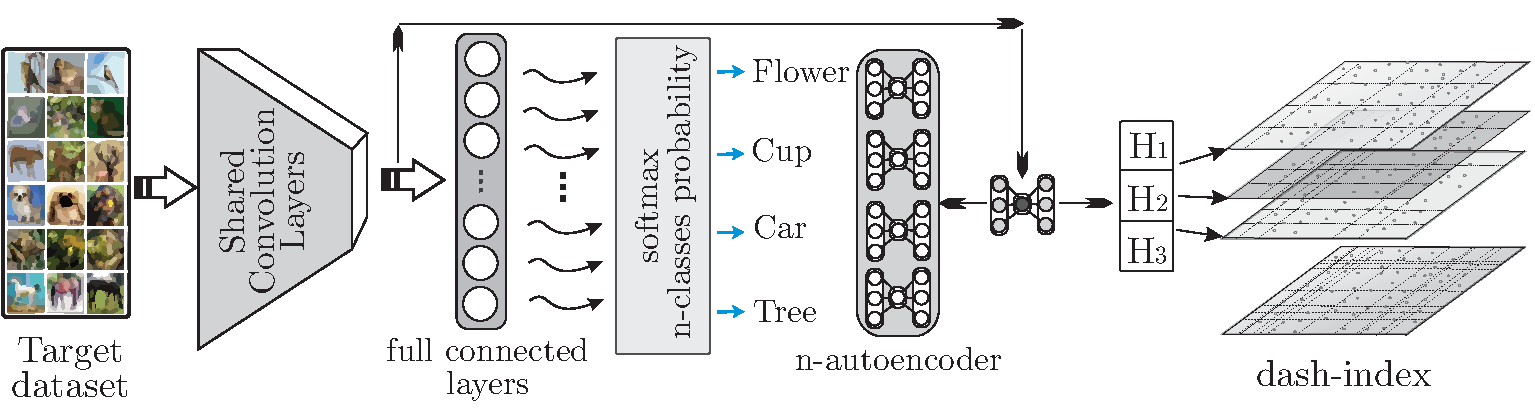
\includegraphics[width=1.0\columnwidth]{dash/DAsh_learning_final.pdf}
\caption{ DAsH. Proceso de entrenamiento e indexación. } 
\label{fig:dash}
\end{figure} 		

Como se mostró en \cite{citeulike:fractal:encoders} un algoritmo de reducción de dimensionalidad exitoso proyecta los datos en un espacio de características con dimensionalidad cercana a la dimensionalidad fractal (FD) de los datos en el espacio original y conserva las propiedades topológicas.  Por lo tanto, para encontrar la dimensionalidad objetivo ($m$) que necesitan las redes de autoencodificadores seguimos la siguiente heurística.  Empezamos con el valor $m_1 = 2^2$, calculamos la FD del nuevo espacio con sólo eso, luego incrementamos el valor en $m_2 = 2^3$, recalculamos la FD, y continuamos haciendo esto hasta algún $ t\ (m_t =  2^t)$ donde podemos ver una mejora en la dimensión fractal, lo que significa que más características no cambian la dimensionalidad fractal del conjunto de datos.
 

El segundo paso de nuestro procedimiento es la recuperación de la imagen vía  DAsH. Procesamos la imagen de consulta enviándola a través de CNN con el objetivo de obtener las clases $n$ más fuertes. En contraste con los algoritmos de aprendizaje de similitud existentes que aprenden la similitud de la característica de bajo nivel, nuestra similitud es la combinación de similitud semántica y nivel de hashing. Así que, la similitud de nivel semántico se calcula en primer lugar. Después de la comprobación de relevancia semántica, obtendremos las nuevas consultas ($q_1, q_2, ... q_n$) usando los  $n$ autoencoders más fuertes. La consulta es transformada en una nueva consulta de objetos ($q_1, q_2, ... q_n$) los cuales son escogidos para localizar los apropiados \textit{buckets}. Una vez que los \textit{buckets} son localizados, el conjunto de candidatos relevantes son formados.  Luego, los elementos del conjunto candidato se analizan exhaustivamente con el fin de recuperar sólo los objetos que satisfacen la condición de consulta. Este proceso es realizado para cada una de las  $L$ tablas hash . Este proceso es ilustrado en la Figura \ref{fig:qdash}.  
\begin{figure}[htp]\centering
\label{fig:qdash}
 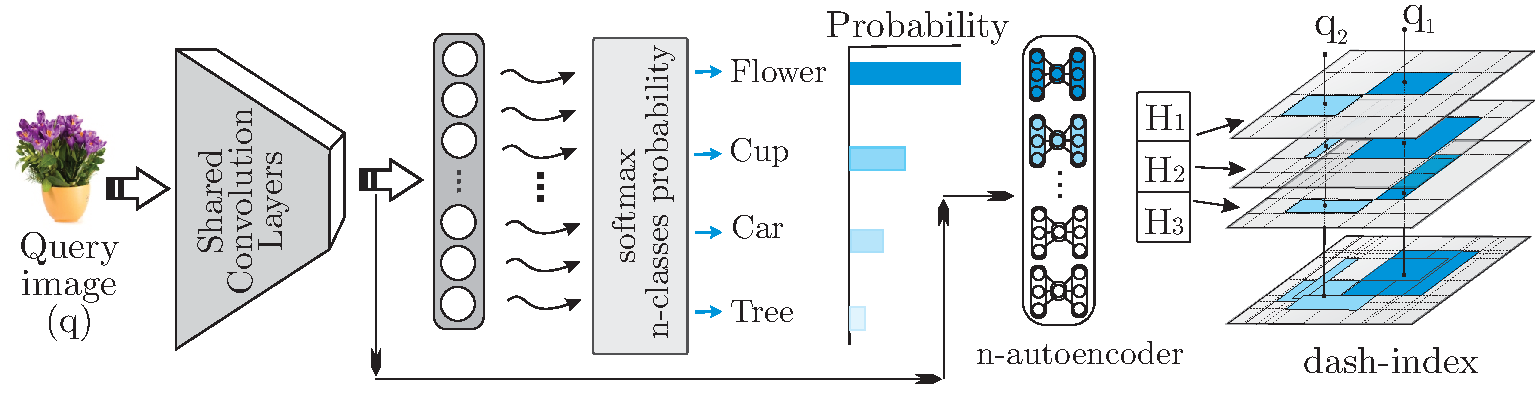
\includegraphics[width=1.00\columnwidth]{dash/DAsh_retrieval_final.pdf} 
\caption{ DAsH.Proceso de recuperación. } 
\end{figure}
 
 
 \subsection{Usando Fractales para estimar los parámetros LSH}
 

La idea de utilizar la Dimensión Fractal de Correlación para calcular los parámetros de LSH se aprovecha en una de las principales características de la Dimensión Fractal de Correlación $\mathfrak{D}$ que aseguran una distribución de la distancia entre los elementos del dataset original y una proyección óptima del sub-espacio se mantiene.  Además, la correlación dimensión fractal $\mathfrak{D}$ se puede estimar en tiempo lineal como se representa en \cite{Faloutsos:2000:SJS:335191.335412}  y \cite{traina2010fast}.  El exponente de distancia $\mathfrak{D}$ tal como está representado en \cite{Faloutsos:2000:SJS:335191.335412} es.
	\begin{equation}\label{eq:logpc_fractal}
	   log(PC(r)) = \mathfrak{D} \times log (r) + K_p 		
	\end{equation}
	
La ecuación \ref{eq:logpc_fractal} usa el número de pares PC(r) con una distancia $r$, pero nosotros estamos interesados en el número de  $k$ elementos involucrados, así que debemos ser capaces de convertir el número de elementos en números de pares dentro de una distancia \cite{Arantes_thefractal}. Por lo tanto, podemos aproximar el radio $r$ usando las ecuaciones anteriores, teniendo en cuenta la correlación de distancia entre el conjunto de datos el número medio de $k$ vecinos dentro de una distancia dada $r$, la aproximación de radio se define como:

\begin{equation}\label{eq:fractalR}
  r  =  R \cdot  exp (  \frac{log (Pairs (k)) - log (Pairs(N))}{ \mathfrak{D} } )    
\end{equation}
Como se representa en \cite{Arantes_thefractal}.   usando la última ecuacion \ref{eq:fractalR} nosotros encontramos el número óptimo de funciones hash $m$  para \acf{LSH} configurado para recuperar el $k$ vecino más cercanos , el cual es proporcional al número de pares a distancia $r$. Esto tiene sentido porque un número medio de $k$ vecinos dentro de una distancia dada $r$. Entonces definimos:
\begin{equation}\label{eq:optimalM1}
   m \approx log (PC(r)) 
\end{equation}
 
 combinando las ecuaciones \ref{eq:optimalM1} y \ref{eq:fractal} obtenemos: $m \approx \mathfrak{D} \cdot log (r)  $.Experimentalmente, confirmamos que el valor óptimo de $m$ es:

 \begin{equation}\label{eq:fractalm}
    m = (\left\lceil \mathfrak{D} + 1 \right\rceil  ) \cdot  log (r)
 \end{equation}
 
\section{Experimentos}

En esta sección, estamos interesados en responder a la siguiente pregunta: (a) ¿Qué tan preciso es nuestro modelo en la estimación de los parámetros LSH utilizando la dimensión fracta?l; (B) ¿Cómo mejora nuestro método DAsH las otras implementaciones de LSH en términos de \textit{consultas de rendimiento} y \textit{precisión}?. El rendimiento del método DAsH se comparó con los de los dos métodos más conocidos, llamado Multi-probe LSH \cite{multiprobe} y LSH-Forest \cite{lshforest}. Todos los experimentos se realizaron en un workstation con Intel core i7  3.0Ghz (12 núcleos) CPU y 64Gb de RAM con cuatro tarjetas gráficas Geforce GTX 1080 GPU de 8Gb VRAM cada una.
 
Primero realizamos experimentos en ocho conjuntos de datos ampliamente utilizados usando características hechas a mano (AUDIO, CITIES, EIGENFACES, HISTOGRAMS, MGCOUNTY, RANDOMWALK, SYNTH16D, SYNTH6D, VIDEO) \footnote{\url{https://github.com/joselhuillca/fractal_dataset}} para evaluar nuestro método propuesto para estimar los parámetros LSH. Además de las características hechas a mano, también mostramos la eficacia de nuestros métodos cuando las características son extraídas por las Redes Neuronales Convolucionales profundas (CNN), realizamos este experimento en tres conjuntos de datos (MNIST\footnote{\url{http://yann.lecun.com/exdb/mnist/}}, CIFAR-10\footnote{\url{https://www.cs.toronto.edu/~kriz/cifar.html}}, SVHN\footnote{\url{http://ufldl.stanford.edu/housenumbers/}}) para evaluarlos en términos de \textbf{consultas de rendimiento} y \textbf{mean average precision (mAP)}. A continuación se describen los detalles de los experimentos y resultados.

\subsection{Experimento 1: Sintonización de parámetros LSH}

Los métodos basados en LSH reportan resultados eficientes cuando los valores $m$ (número de funciones hash) son elegidos.Para evaluar la eficacia del enfoque presentado para afinar los parámetros LSH utilizando la dimensión fractal, hemos trabajado en una variedad de datos sintéticos y reales. Tabla \ref{table:lshparams} resume las principales características y parámetros de los conjuntos de datos, incluyendo el número de elementos $N$, el número de atributos $d$, su dimensión intrínseca (fractal) $D$ y los parámetros LSH usando dos aproximaciones: el algoritmo de Andoni \footnote{\url{http://www.mit.edu/~andoni/LSH/}}  y nuestra propuesta basada en dimension fractal.  os resultados del experimento para el número de funciones de hash $m$ muestran que las estimaciones dadas por la ecuación \ref{eq: fractalm} son comparables con las obtenidas con el algoritmo E2LSH propuesto por Andoni utilizando hasta 10 veces menos tiempo.
 
\begin{table}[!t]
\caption{Parametros óptimos LSH, utilizando e2lsh exhaustivo y el método basado en fractales. **Tiempo en segundos. }
\label{table:lshparams}
\centering
\begin{footnotesize}
\begin{tabular}{c|r|r|r|r|r|r|r|r|r|r|}
    \cline{2-11}
    & \multicolumn{ 2}{|c|}{{\bf dataset}} & \multicolumn{ 3}{|c|}{{\bf fractal params}} & \multicolumn{ 2}{|c|}{{\bf e2lsh}} & \multicolumn{ 3}{|c|}{{\bf fractalsh}}  \\
    \cline{2-11}
    & \multicolumn{1}{c|}{$N$}    & \multicolumn{1}{c|}{$d$} & \multicolumn{1}{c|}{$D$}    & $log(R)$ & $log(CR)$   & $m$ & \multicolumn{1}{c|}{$time$}    & \multicolumn{1}{c|}{$r$}  & $m$ & \multicolumn{1}{c|}{$time$} \\
    \hline
\multicolumn{1}{|c|}{\bf audio}                 & 54387                 & 192      & 6.49     & -1.30      & 17.00       & 18                        & 64.20     & 0.14  & 16                    & 12.68                   \\
\multicolumn{1}{|c|}{\bf cities}                & 5507                  & 2        & 2.36     & 2.30       & 16.00       & 8                         & 16.45      & 4.16  & 6                     & 0.81                    \\
\multicolumn{1}{|c|}{\bf eigenfaces}            & 11900                 & 16       & 4.25     & -1.40      & 18.00       & 12                        & 42.28      & 0.13  & 13                    & 1.57                    \\
\multicolumn{1}{|c|}{\bf histograms}            & 4247                  & 256      & 2.50     & -0.81      & 16.01       & 6                         & 15.62      & 0.22  & 7                     & 6.12                    \\
\multicolumn{1}{|c|}{\bf mgcounty}              & 27282                 & 2        & 1.81     & 0.70       & 19.00       & 4                         & 87.96      & 0.27  & 4                     & 1.13                     \\
\multicolumn{1}{|c|}{\bf randomwalk}            & 10000                 & 1024     & 5.52     & 2.80       & 15.00       & 16                        & 50.60     & 10.16 & 17                    & 10.60                   \\
\multicolumn{1}{|c|}{\bf synth16d}              & 10000                 & 16       & 8.36     & -1.40      & 17.00       & 20                        & 27.20     & 0.18  & 18                    & 7.51                   \\
\multicolumn{1}{|c|}{\bf synth6d}               & 10000                 & 6        & 4.95     & -1.40      & 17.00       & 12                        & 28.16      & 0.14  & 12                    & 6.47                    \\
\multicolumn{1}{|c|}{\bf video}                 & 79094                 & 50       & 7.73     & -1.40      & 21.00       & 16                        & 1205.73     & 0.13  & 19                    & 92.54                   \\ 
\bottomrule
\end{tabular}
\end{footnotesize}
\end{table}
Gracias a esta relación entre los parámetros LSH y la dimensión fractal, podemos trabajar con datos a gran escala. Además, debido a la dimensión fractal se puede estimar en tiempo lineal podemos estimar óptimamente los parámetros de LSH en tiempo lineal también. 

\subsection{Rendimiento de Recuperación} % OK
El objetivo de este experimento es medir el tiempo total dedicado a preparar el índice y recuperar los objetos vecinos más cercanos de un conjunto de datos usando consultas k-neighbor más cercanas $ kNNq $. Las estructuras de datos que se compararon se probaron con valores específicos para las consultas. Por lo tanto, usamos $ k = 1000 $ para las consultas $ kNN $.

\begin{table}[ht]
\caption{Mean Average Precision(mAP) y el tiempo acumulado dedicado a calcular mAP para diferentes métodos en los conjuntos de datos MNIST, SVHN y CIFAR-10. ** Tiempo en segundos.  }
\label{table:map}
\centering
\begin{footnotesize}
\begin{tabular}{l|c|c|c|c|c|c|c|c|c|}
\cline{2-10}
                                           & \multicolumn{3}{c|}{\textbf{MNIST}}            & \multicolumn{3}{c|}{\textbf{SVHN}}             & \multicolumn{3}{c|}{\textbf{CIFAR-10}}         \\ \cline{2-10} 
                                           & \textbf{mAP} & \textbf{P (\%)} & \textbf{time} & \textbf{mAP} & \textbf{P (\%)} & \textbf{time} & \textbf{mAP} & \textbf{P (\%)} & \textbf{time} \\ \hline
\multicolumn{1}{|l|}{\textbf{MpLSH \cite{multiprobe}}}       & 0.86         & 0.95            & 19.58         & 0.71         & 0.73            & 8.09          & 0.83         & 0.89            & 122.45        \\ \hline
\multicolumn{1}{|l|}{\textbf{ITQ \cite{itq}}}         & 0.87         & 0.95            & 1297.32       & 0.70         & 0.80            & 8411.26       & 0.84         & 0.88            & 1056.83       \\ \hline
\multicolumn{1}{|l|}{\textbf{LOPQ \cite{lopq}}}        & 0.86         & 0.90            & 119.21        & 0.71         & 0.74            & 613.65        & 0.83         & 0.88            & 528.20        \\ \hline
\multicolumn{1}{|l|}{\textbf{LSH-F \cite{lshforest}}}       & 0.85         & 0.96            & 217.33        & 0.61         & 0.78            & 365.90        & 0.86         & 0.89            & 365.47        \\ \hline
\multicolumn{1}{|l|}{\textbf{DAsH (Ours)}} & 0.93         & 0.98            & 20.82         & 0.74         & 0.84            & 10.34         & 0.88         & 0.91            & 125.37        \\ \hline
\end{tabular}
\end{footnotesize}
\end{table}
La Tabla  \ref{table:map} muestra la comparación en términos de mean average precision (mAP)  y tiempo de consulta para todos los métodos basados en hash. El método DAsH fue significativamente mejor que otros métodos; proporcionando hasta un mAP 10 \% mejor,  manteniendo un excelente tiempo de recuperación. Este resultado demuestra el potencial de impulsar las operaciones de consulta con el diseño de estructuras de índices especializados.


